\begin{frame}{Motivation}

\frametitle{Motivation}
Bound $b\bar{b}$ states, which can be produced in different spin
configurations, are an ideal laboratory for QCD tests. It's like a hydrogen
atom in QCD.
\begin{columns}[c]
\column{.4\textwidth}
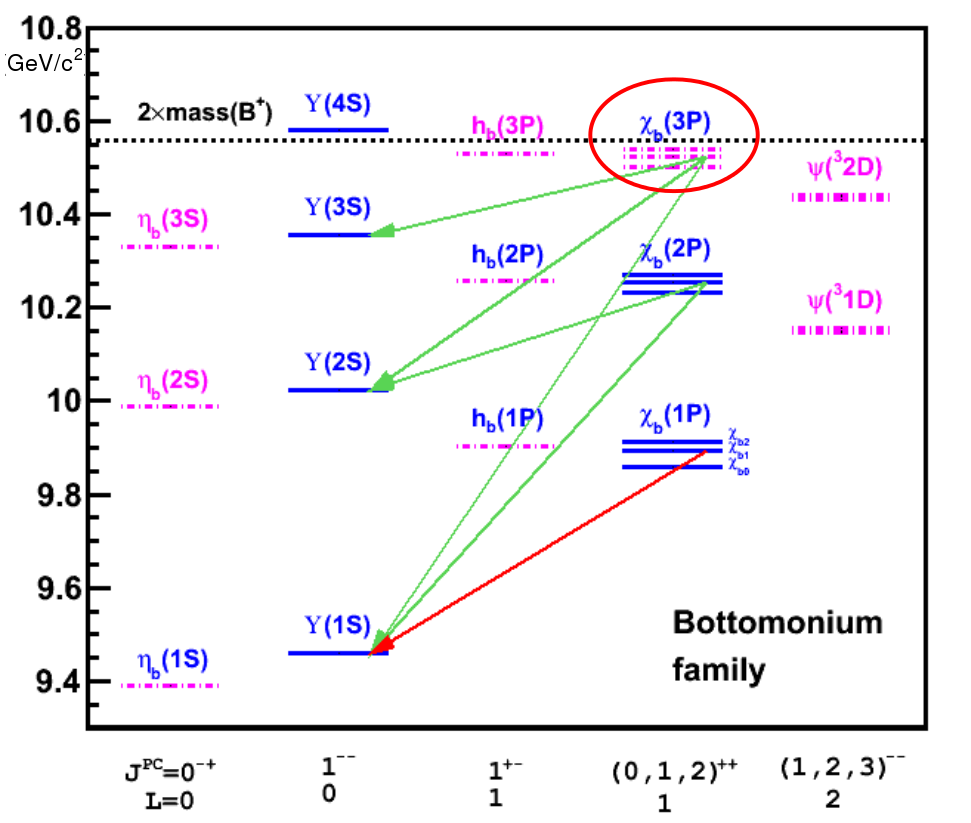
\includegraphics[width=\textwidth]{bfamily.png}
\begin{itemize}
  \item \textcolor{blue}{Measured mass}
  \item \textcolor{red}{Mass from theory}
\end{itemize}
\column{.6\textwidth}
\fontsize{9pt}{7.2}\selectfont
States with parallel quark spins (S=1):
\begin{itemize}
  \item S-wave $\Upsilon$ state.
  \item P-wave $\chi_{b}$ states, composed by 3 spin states $\chi_{b(0,1,2)}$. 
  \item $\Upsilon$ can be readily produced in the radiative decays of $\chib$.
  \item $\chi_{b}(3P)$ state recently observed by ATLAS, D0 and LHCb.
\end{itemize}
\textcolor{red}{This thesis:}
\begin{enumerate}
  \item Measurement of  $\Upsilon(NS)$ (N=1, 2, 3) fraction  originating from \chib decays
  \item Measurement of $\chi_{b}(3P)$ mass.
\end{enumerate}
\end{columns}

\end{frame}